\chapter{Manual d'usuari}
\label{cha:userguide}
En aquest apendix es dona una descripcio de com accedir als recursos i com fer funcionar la aplicacio.

\section{Introducció}
La aplicació esta dissenyada per instal·lar-se en qualsevol servidor i la ruta de accés principal depen de la instal·lació.
Si la aplicació esta en local, normalment l'accés es faria des de el navegador amb la URL http://localhost/login per introduir les credencials i entrar a la aplicació o per crear-se una compte.\\

Una vegada autenticat el sistema, a la part superior el menú sempre serà visible i la seva estructura esta explicada a la secció \ref{subsec:maindessign} a la p\`{a}gina \pageref{menudessign}.

\section{Casa de l'usuari}
\label{sec:home}
Per accedir la casa de l'usuari(figura \ref{fig:dashboard}) es pot fer mitjançant el logo de ''Ichnaea'' del menú situat a l'esquerra.\\

\begin{figure}[h!]
  \centering
  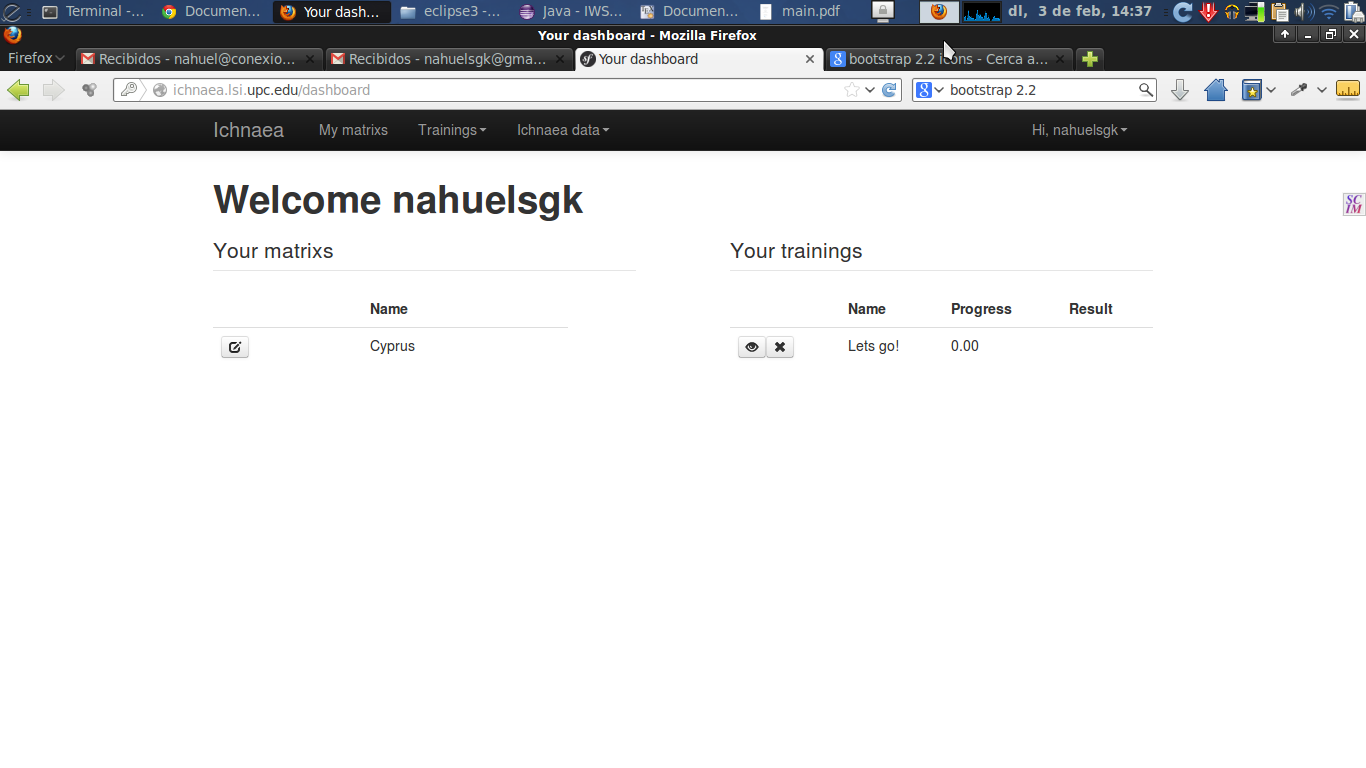
\includegraphics[scale=0.4]{img/userguide/dashboard.png}
  \caption{Interfície d'usuari: ''Casa de l'usuari''}
  \label{fig:dashboard}
\end{figure}

A continuaci\'{o} descriurem cadascuna de les parts.

\subsection{Llistat dels meus entrenaments pendents}
Al llistat superior(''My pending trainings'') pots veure els entrenaments que has creat i que estan pendents de finalitzar, on: 
\begin{itemize}
\item Nom del entrenament.
\item Nom de la matriu entrenada com a enllaç per veure la matriu.
\item Descripci\'{o} del entrenament.
\item Origen: Paràmetre de creació seleccionat per l'entrenament. Actualment solament es guarda el valor però Ichnaea no esta desenvolupat encara per executar un entrenament amb aquest paràmetre.
\item Data de creaci\'{o} de l'entrenament.
\item Nom de l'usuari que la creat(que sempre serà l'usuari registrat).
\item Progr\'{e}s: actualment Ichnaea no retorna estat del proces. Solament ens diu si ha acabat o no. Per tant els \'{u}nics valors son 0.00 i 1.00.
\item Status. Els possibles estats son ''pending''(no s'ha pogut enviar),''sent''(s'ha enviat a la cua). Els entrenaments finalitzats es poden consultar a ''Els meus entrenaments''. A la secció \ref{subsec:myTrainings} es dona mes informació al respecte.
\item Error: en cas que hi hagués algun error en el entrenament des de Ichnaea, sortiria un breu descripció.(secció  \ref{sec:ichnaeaErrors})
\item Operacions
 \begin{itemize}
 \item \iconeyeopen es per anar a la pantalla de visualització de l'entrenament.
 \end{itemize}
\end{itemize}

\subsection{Llistat de les meves prediccions pendents}
Al llistat inferior(''My pending predictions'') pots veure les prediccions que has creat i que estan pendents de finalitzar, on: 
\begin{itemize}
\item Nom de la predicció.
\item Nom de la matriu entrenada com a enllaç per veure la matriu.
\item Descripci\'{o} del entrenament que s'esta usant en la predicció.
\item Origen: Paràmetre de creació seleccionat per l'entrenament. Actualment solament es guarda el valor pero Ichnaea no esta desenvolupat encara per executar una entrenament amb aquest paràmetre.
\item Data de creaci\'{o} de la predicció.
\item Nom de l'usuari que la creat(que sempre serà l'usuari registrat).
\item Status. Els possibles stats son ''pending''(no s'ha pogut enviar),''sent''(s'ha enviat a la cua). Els entrenaments finalitzats es poden consultar a ''Els meus entrenaments''(mirar \ref{subsec:myPrediccions}).
\item Error: en cas que hi hagués algun error en el entrenament des de Ichnaea, sortiria un breu descripció. A la secció Mirar \ref{sec:ichnaeaErrors} es dona mes informació al respecte.
\item Operacions
 \begin{itemize}
 \item \iconeyeopen es per anar a la pantalla de visualització de l'entrenament.
 \end{itemize}
\end{itemize}

\subsection{Els meus entrenaments}
\label{subsec:myTrainings}
Per accedir als teus entrenaments, accedir al menú ''Trainings >> My trainings''. A la figura \ref{fig:my_trainings} es pot veure el llistat els entrenaments d'un usuari on:
\begin{figure}[h!]
  \centering
  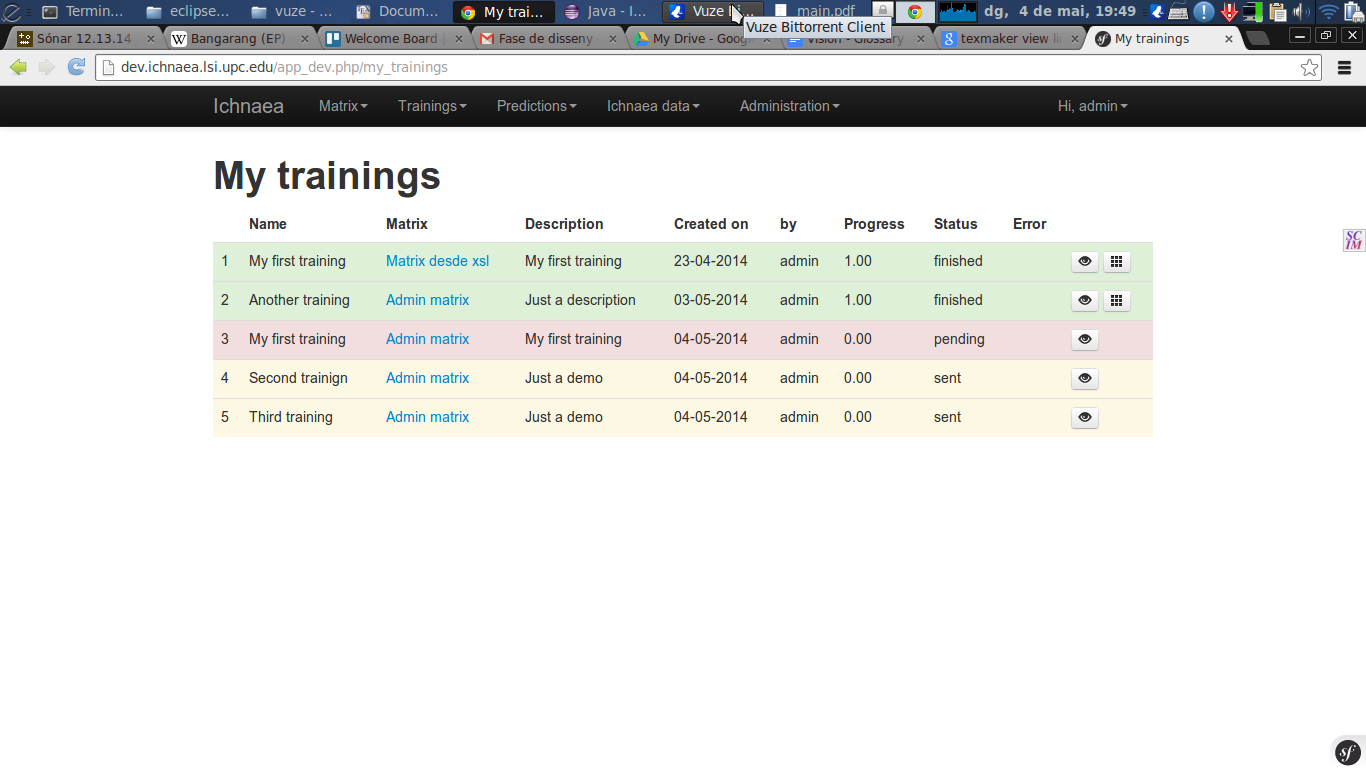
\includegraphics[scale=0.4]{img/userguide/my_trainings.png}
  \caption{Interfície d'usuari: ''Els meus entrenaments''}
  \label{fig:my_trainings}
\end{figure}

\begin{itemize}
\item Nom del entrenament.
\item Nom de la matriu entrenada com a enllaç per veure la matriu.
\item Descripci\'{o} del entrenament.
\item Origen: Paràmetre de creació seleccionat per l'entrenament. Actualment solament es guarda el valor pero Ichnaea no esta desenvolupat encara per executar un entrenament amb aquest paràmetre.
\item Data de creaci\'{o} de l'entrenament.
\item Nom de l'usuari que la creat(que sempre serà l'usuari registrat).
\item Progr\'{e}s: actualment Ichnaea no retorna estat del proces. Solament ens diu si ha acabat o no. Per tant els \'{u}nics valors son 0.00 i 1.00.
\item Status. Els possibles status son ''pending''(no s'ha pogut enviar),''sent''(s'ha enviat a la cua) i ''finished''(finalitzat). 
\item Operacions
 \begin{itemize}
 \item \iconeyeopen per accedir a la pantalla de visualització de l'entrenament.
 \end{itemize}
\end{itemize}

\subsection{Les meves prediccions}
\label{subsec:myPrediccions}
Per accedir a les teves prediccions, accedir al menú ''Predictions >> My predictions''. A la figura \ref{fig:my_predictions} es pot veure el llistat de les prediccions d'un usuari on:
\begin{figure}[h!]
  \centering
  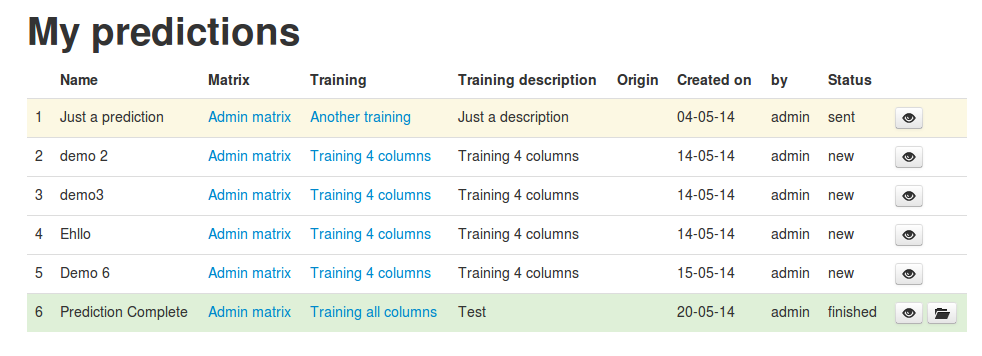
\includegraphics[scale=0.4]{img/userguide/my_predictions.png}
  \caption{Interfície d'usuari: ''Les meves prediccions''}
  \label{fig:my_predictions}
\end{figure}
\begin{itemize}
\item Nom de la predicció.
\item Nom de la matriu entrenada com a enllaç per veure la matriu.
\item Nom de l'entrenament com a enllaç per veure quin entrenament s'esta usant per la predicció.
\item Descripció de l'entrenament que s'esta usant en la predicció.
\item Origen: Paràmetre de creació seleccionat per l'entrenament. Actualment solament es guarda el valor pero Ichnaea no esta desenvolupat encara per executar una entrenament amb aquest paràmetre.
\item Data de creaci\'{o} de la predicció.
\item Nom de l'usuari que la creat(que sempre serà l'usuari registrat).
\item Status. Els possibles status son ''pending''(no s'ha pogut enviar),''sent''(s'ha enviat a la cua), ''finished''(ha finalitzat) i ''new''(s'esta configurant encara la matriu de predicció).
\item Error: en cas que hi hagues algun error en el entrenament desde Ichnaea, sortiria un breu descripcio. A la secció \ref{sec:ichnaeaErrors} es dona m\'{e}s informació al respecte.
\item Operacions
 \begin{itemize}
 \item \iconeyeopen per accedir a la pantalla de visualització de l'entrenament.
 \item \iconresults per consultar els resultats.
 \end{itemize}
\end{itemize}

\section{Variables}
\subsection{Veure les variables del sistema}
Desde el menu ''Ichnaea  Data - View Variables'', es poden veure totes les variables del sistema. Amb la icona \iconeyeopen, es pot accedir a la interfície de configuraci\'{o} de la variable seleccionada.

\subsection{Formulari de edici\'{o} d'una variable}
\begin{figure}[h!]
  \centering
  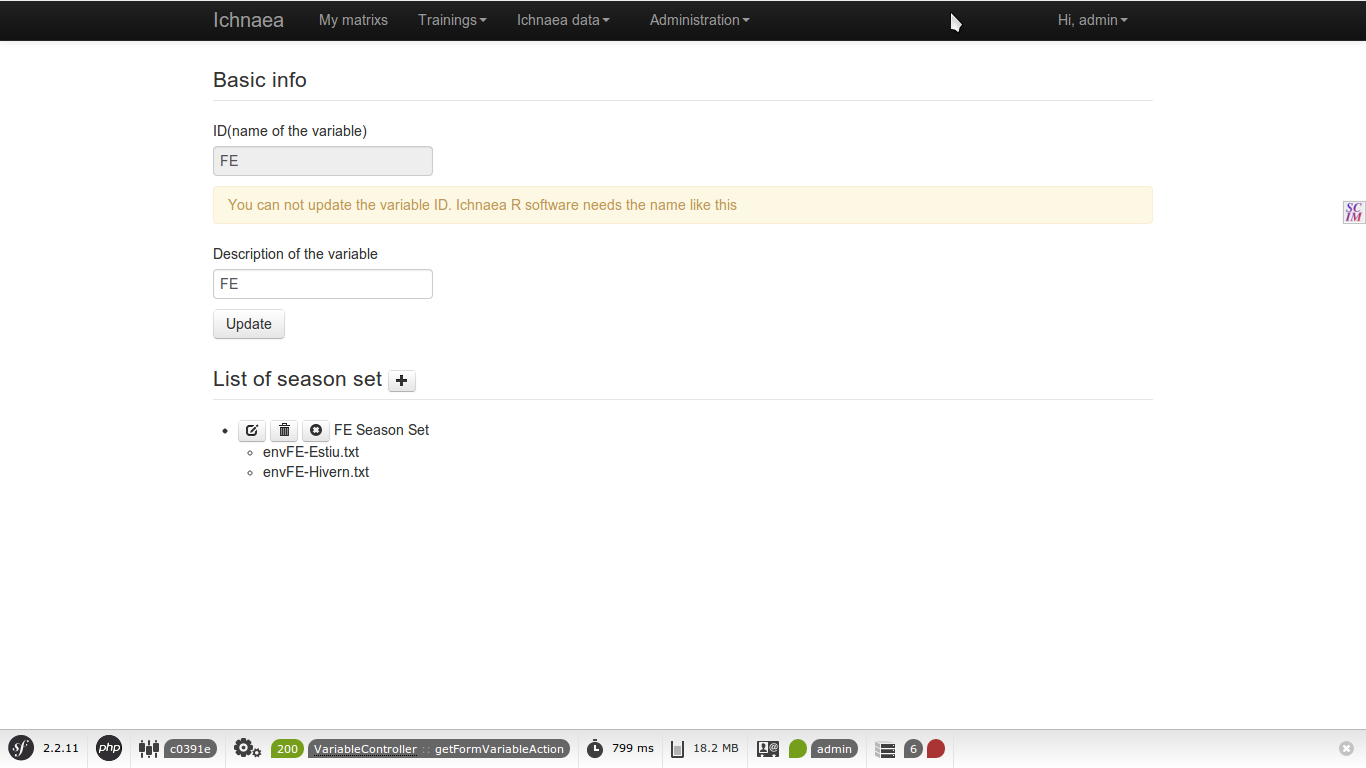
\includegraphics[scale=0.5]{img/userguide/variable_configuration.png}
  \caption{Interfície de configuraci\'{o} d'una variable}
  \label{fig:placement}
\end{figure}
A continuació es descriuen les parts bàsiques d'aquest formulari.

\subsection*{Informació bàsica}
L' ID \'{e}s l'identificador d'Ichnaea i la descripció \'{e}s un camp modificable per descriure la variable.
\subsection{Llistat de conjunts de fitxers}
A l'apartat ''List of season set'' es veuen els conjunts de fitxers amb el seus components d'aquesta variable on:
\begin{itemize}
\item \iconedit per modificar el conjunt de fitxers(nom, components i configuracions).
\item \icontrash per esborrar tot el conjunt i tots el fitxers associats, excepte els compartits(simplement esborra la associació).
\item \iconadd per afegir un conjunt nou de fitxers
\end{itemize}

\subsection{Formulari de creació i d'actualització d'un conjunt de fitxers(''Season set'')}
A la figura \ref{fig:seasonSetEdition} es pot veure aquest formulari.
\label{season_set:variable}
\begin{figure}[h!]
  \centering
  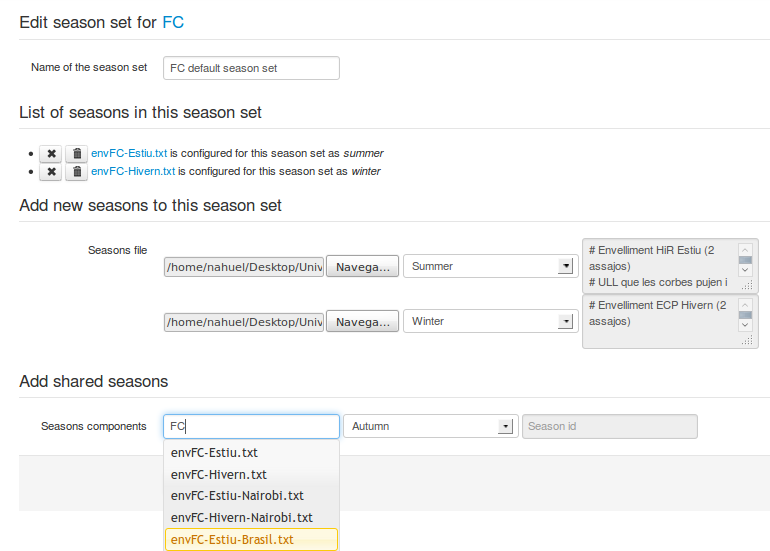
\includegraphics[scale=0.5]{img/userguide/season_set_edition.png}
  \caption{Interfície de configuraci\'{o} de conjunts de fitxers d'una variable}
  \label{fig:seasonSetEdition}
\end{figure}
A continuació es descriuen les funcionalitats d'aquest formulari.

\subsubsection{Afegir nous fitxers a un conjunt de fitxers}
A l'apartat \textbf{''Add new seasons to this season set''}, \'{e}s pot afegir nous fitxers localitzats a la maquina de l'usuari amb un navegador típic de fitxers accedint a ''Navega...''. \\

El selector de temporades es per configurar el fitxer com estiu, hivern, tardor, primavera o com a tot l'any.\\

El tercer camp \'{e}s un camp especial de tipus ''sols lectura'' per comprovar que el fitxer es carrega be.\\

Actualment el format del fitxer que accepta Ichnaea, es un fitxer de text amb la estructura que es veu a la figura \ref{fig:envelliment}. Les línies que comencen per '\#' son línies que Ichnaea escapa.

\begin{figure}[h!]
  \centering
  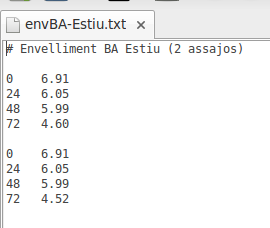
\includegraphics[scale=0.5]{img/userguide/envelliment.png}
  \caption{Format d'un fitxer d'envelliment}
  \label{fig:envelliment}
\end{figure}

\subsubsection{Afegir un fitxer d'una altre variable}
En el cas de que existeixin variables que tinguin envelliments similars, es pot buscar a la secció ''Add shared seasons''.\\

\'{E}s un camp de tipus auto-completat que desplega un menú per que l'usuari seleccioni el que busca. Amb el següent selector el pot configurar. L'ultim camp es per comprovar que el fitxer es carrega be.

\subsubsection{Esborrar un fitxer del conjunt de fitxers}
Amb la icona \icontrash pots esborrar el fitxer i el seu contingut d'aquest conjunt de fitxers.\\
Amb la icona \iconremove pots esborrar el fitxer com a component. Per exemple, si has afegit un fitxer compartit, no esborres el fitxer sinó que simplement deixa de estar associat a aquest conjunt de fitxers.

\section{Matrius}

\subsection{Crear una matriu desde un fitxer CSV o Excel}
\label{sec:create_matrix}
Desde el menu superior ''IchnaeaData - New matrix'', es pot pujat una nova matriu en format CSV o Microsoft Excel. El format CSV es compatible amb les programaris de ofim\`{a}tica m\'{e}s habituals como Microsoft Excel o Libreoffice.

El format del fitxer de la matriu \'{e}s com es mostra a la figura \ref{fig:matrixSource}.
\begin{figure}[h!]
  \centering
  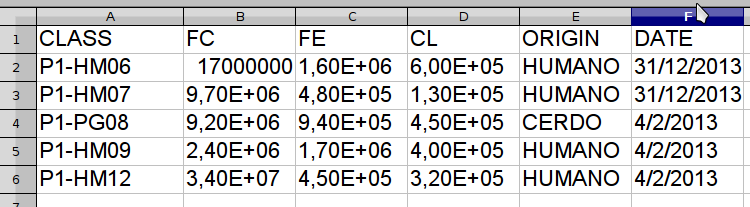
\includegraphics[scale=0.5]{img/userguide/matrix_source.png}
  \caption{Fulla de calcul d'exemple}
  \label{fig:matrixSource}
\end{figure}

\begin{itemize}
\item Primera columna. Son els identificadors de la variable. Si una columna es diu igual que una variable del sistema, automàticament s'assigna a aquesta variable.
\item Les ultimes dues columnes son especials i son opcionals. Es contemplen totes les casuístiques:
\begin{itemize}
\item No existeixen
\item Solament ORIGIN
\item Solament DATE
\item Primer ORIGIN i després DATE
\item Primer DATE i després ORIGIN
\end{itemize}
\item La columna ORIGIN explicita l'origen de les mostres. En el cas que no sigui present, cada mostra s'intentar\`{a} resoldre  amb un associació segons sub-cadenes:
\begin{itemize}
\item Si el identificador de la mostra conte HM es resoldrà com HUMAN.
\item Si el identificador de la mostra conte PG es resoldrà com PIG.
\item Si el identificador de la mostra conte PL es resoldrà com POULTRY.
\item Si el identificador de la mostra conte CW es resoldrà com COW
\end{itemize}
\item La columna DATE explicita les dates de les mostres amb el format DD/MM/YYYY.
\end{itemize}

El resultat d'aquest exemple es pot veure a la figura \ref{fig:matrixResulting}:
\begin{figure}[h!]
  \centering
  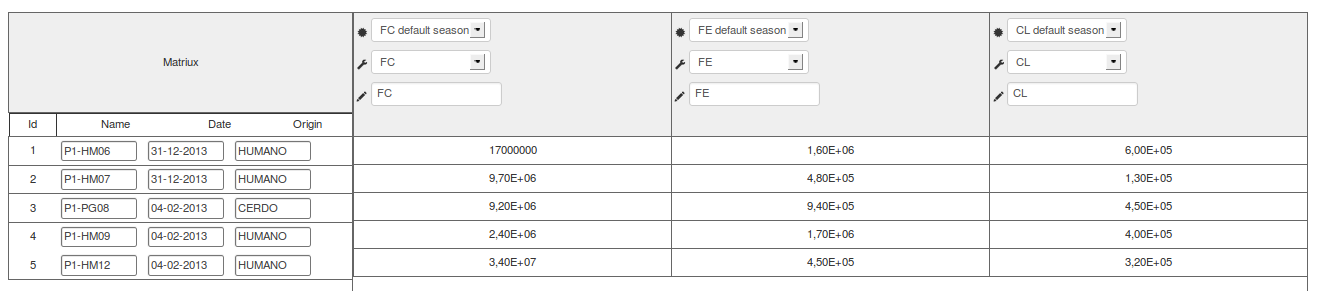
\includegraphics[scale=0.3]{img/userguide/matrix_resulting.png}
  \caption{Resultat de la importació d'una fulla d'exemple}
  \label{fig:matrixResulting}
\end{figure}

\subsection{Interfície de configuració d'una matriu}
\label{subsec:interfaceConfiguration}
A la figura \ref{fig:configure_matrix} es pot veure la interfície de configuració de les matrius.
\begin{figure}[h!]
  \centering
  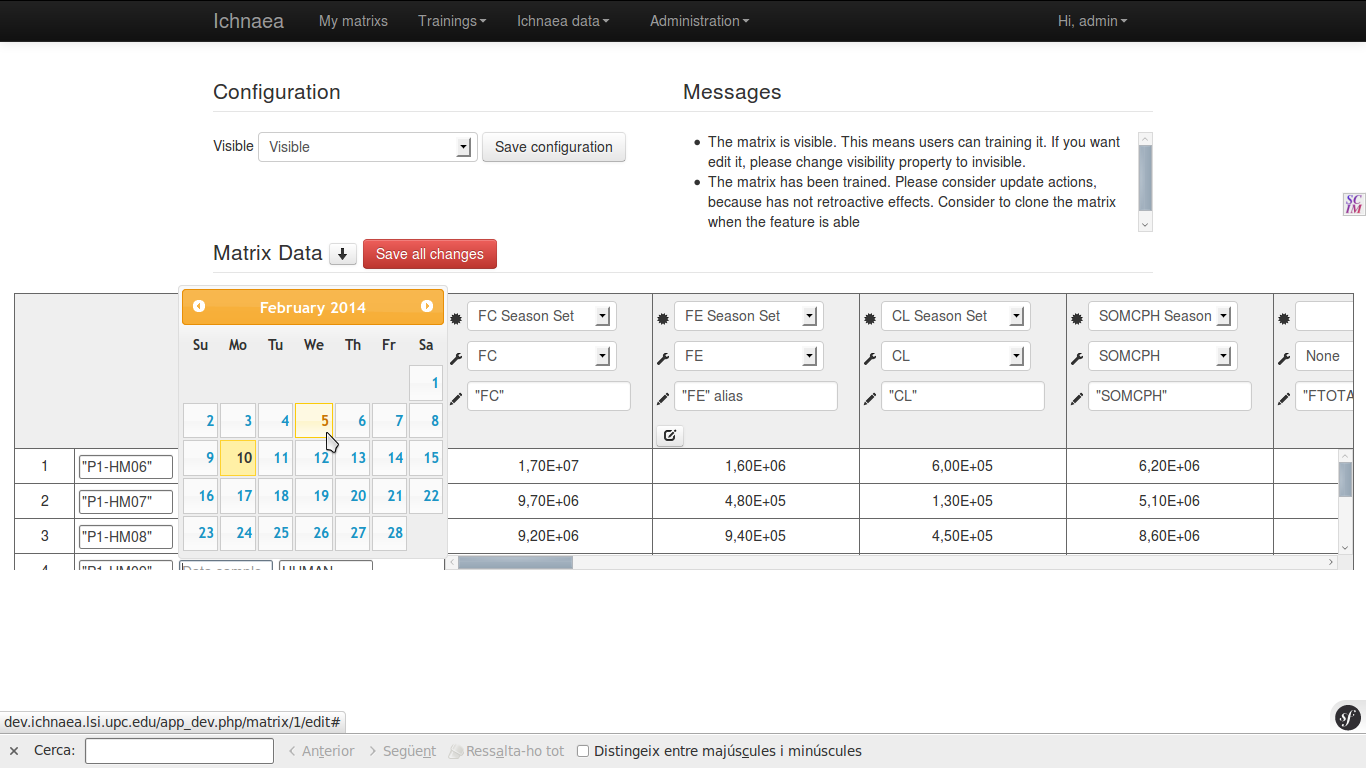
\includegraphics[scale=0.2]{img/userguide/matrix_configure.png}
  \caption{Interfície de configuraci\'{o} de matrius}
  \label{fig:configure_matrix}
\end{figure}

\textbf{Solament l'usuari propietari de la matriu la pot configurar}. A continuació descrivim les seccions de la interfície.
\begin{itemize}
\item Configuració bàsica
\item Missatges
\item Accions
\item Dades de Matrius
\end{itemize}

\subsubsection{Configuració bàsica}
La visibilitat \'{e}s un paràmetre per permetre que altres usuaris vegin la matriu per entrenar-la.

\subsubsection{Missatges} 
Apartat on el sistema comunica a l'usuari errors de validacions i perills.

\subsubsection{Accions} 
Les accions disponibles son:
\begin{itemize} 
\item \icondownload per descarregar-se la matriu en CSV.
\item \iconupdate per actualitzar les dades, no la configuració.
\item \icontrash per esborrar la matriu, els entrenaments i les prediccions
\item \icontraining per crear un entrenament amb aquesta matriu
\item But\'{o} ''Validate'': valida la matriu. Sortiran a la secció de missatges els possibles errors.
\end{itemize}

\phantonsection
\label{matrixConfiguration}
\subsubsection{Configuració de les dades de la matriu}
\paragraph*{Columnes} Des de les columnes, es configuraren les variables de la matriu on:
\begin{itemize}
\item \iconalias es per definir el alies de la columna
\item \iconvariable es per seleccionar una variable. Si no es selecciona res, quedara configurada com una variable derivada.
\item \iconseason en cas de seleccionar una variable, es carregaran els conjunts de fitxers de la variable.
\end{itemize}
Una vegada actualitzat les dades en alguna columna, apareixerà la icona \iconedit per salvar les dades. En el cas que hagi diferents columnes configurades, es podrà pitjar el buto ''Save all changes''.

\paragraph*{Actualitzar una mostra} Per actualitzar una mostra:
\begin{itemize}
\item El primer camp es l'alies de la mostra
\item El segon es un calendari per seleccionar una data
\item El tercer es un camp auto completat optatiu. Quan es comença a escriure, surt un desplegable per seleccionar un dels possibles valors dels orígens que existeixen a la matriu o escriure un nou.
\end{itemize}

\paragraph*{Actualitzar una dada d'una fila i d'una columna} Es poden actualitzar les dades d'una mostra fent un doble ''click'' en una de les celles. Prement ''Enter'' es guarda el resultat.


\subsection{Clonar una matriu}
\label{subsec:clone_matrix}
L'objectiu de clonar una matriu es per tenir matrius similars però per canviar de configuracions. L'objectiu de canviar de configuració es crear entrenaments amb altres configuracions(altres conjunts de fitxers per variable, o modificar un origen , etc). No es copien ni els entrenaments ni les prediccions. Una matriu entrenada no es pot canviar la configuració.\\

Per clonar una matriu, seguir el menú ''Ichnaea Data - View Matrix'', podem accedir al llistat de variables del sistema; amb la icona \iconclone accedim al formulari de clonaci\'{o}(figura \ref{fig:cloneMatrix}). 
\begin{figure}[h!]
  \centering
  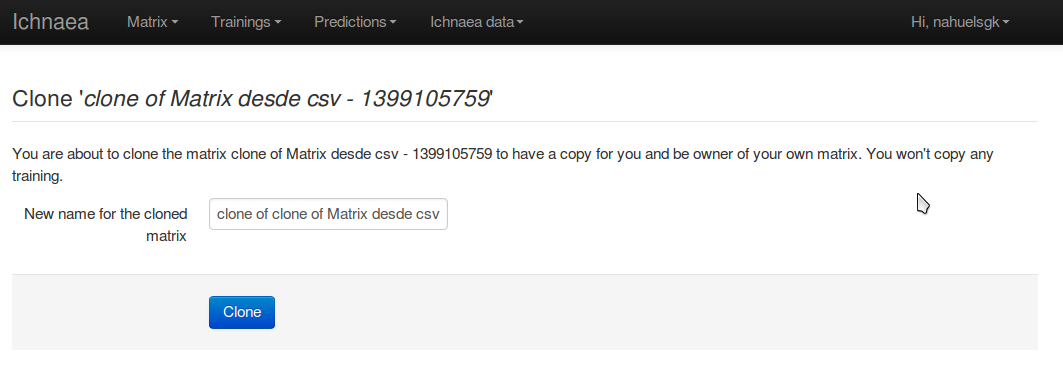
\includegraphics[scale=0.2]{img/userguide/clone_matrix}
  \caption{Interfici d'usuari ''Clonar una matriu''}
  \label{fig:cloneMatrix}
\end{figure}
El formulari suggereix un nom que es pot canviar. Si l'usuari accepta la clonaci\'{o} l'usuari clona les dades i la configuraci\'{o} i es dirigir\`{a} a la la interfície de configuració.


\section{Entrenaments}
\subsection{Crear un entrenament d'una matriu}
\label{subsec:createtraining}
Per crear un entrenament primerament s'ha de seleccionar un matriu. Per crear un entrenament existeixen diferents formes:
\begin{itemize} 
\item Opció 1) Des de el llistat de matrius entrenables(''Ichnaea Data >> Create training'') amb la icona \icontraining.
\item Opció 2) Visualitzant una matriu accedint des de el llistat de matrius del sistema: ''Ichnaea Data >> View matrixs >> \iconeyeopen >> \icontraining.
\item Opcio 3) Des de la interfície de configuració de la matriu(mirar la secció \ref{subsec:interfaceConfiguration}).
\end{itemize}

La figura \ref{fig:createTraining} \'{e}s la interfície de creació d'entrenaments on:
\begin{figure}[h!]
  \centering
  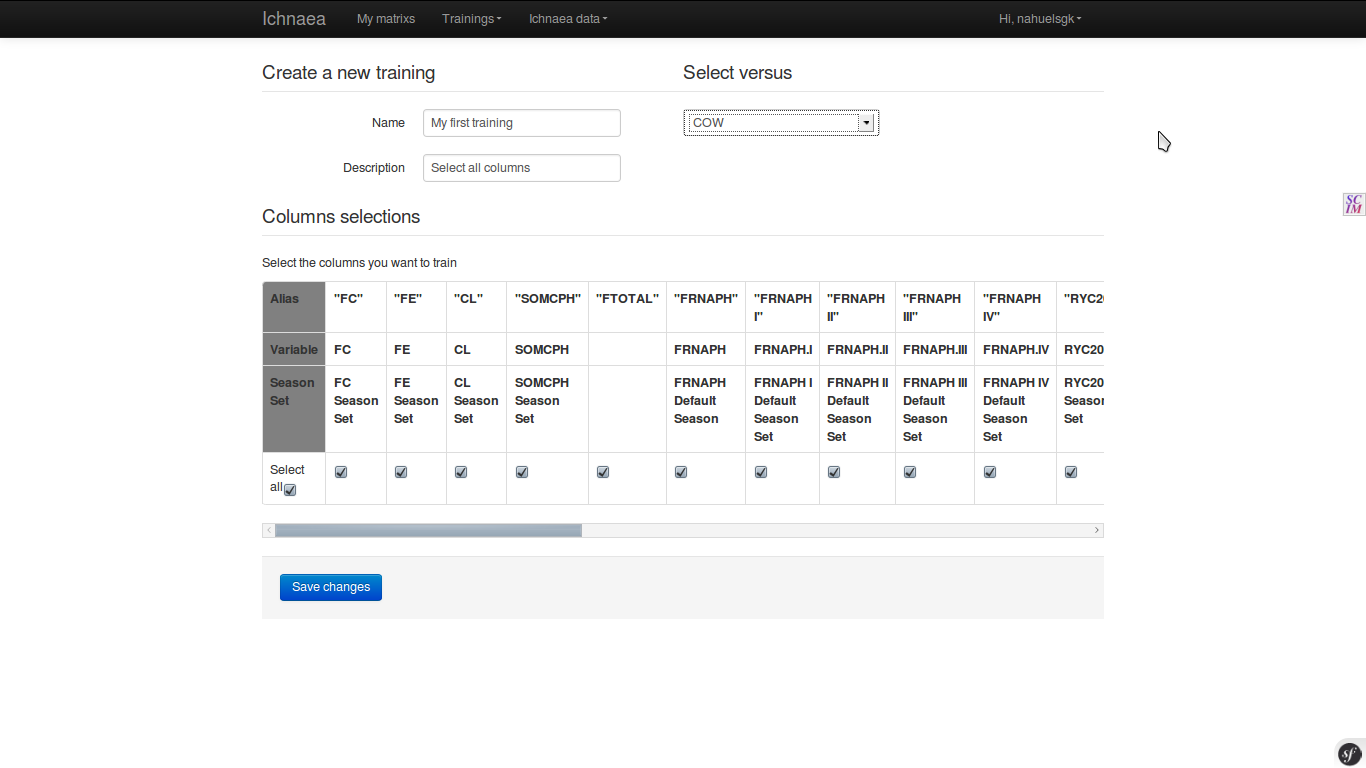
\includegraphics[scale=0.4]{img/userguide/training_create.png}
  \caption{Llistat de matrius}
  \label{fig:createTraining}
\end{figure}
\begin{itemize}
\item Part esquerra superior: nom i descripci\'{o} de l'entrenament.
\item Part dreta superior: Desplegable per seleccionar un dels orígens disponibles.  El ''origen-versus'', es un llistat de la variable origen de la matriu. Si es selecciona el valor "All versus all", l'entrenament ser\'{a} tots contra tots. Si \'{e}s selecciona un origen concret, l'entrenament es far\`{a} aquest origen contra els altres. \textbf{Actualment Ichnaea no suporta aquesta part per\'{o} en el futur est\`{a} planificat que ho far\`{a}}.
\item Selecci\'{o} de columnes. Selecci\'{o} de columnes que vols entrenar.
\end{itemize}

Si la creaci\´{o} \´e{s} correcte, les dades s'enviaran a la cua de procesos i la aplicaci\´{o} es redirigir\´{a} la pantalla de visualitzaci\´{o} de entrenaments(mirar la secció \ref{subsec:viewtraining}).

\subsection{Visualitzar un entrenament}
\label{subsec:viewtraining}
Des de la casa de l'usuari(mirar \ref{sec:home}), es pot veure els teus entrenaments pendents i en quin estadi es troben. Per els finalitzats, es poden accedir des de ''Els meus entrenaments''(secció \ref{subsec:myTrainings}).

La figura \ref{fig:viewTraining} es la interfícies que mostra un entrenament on:
\begin{figure}[h!]
  \centering
  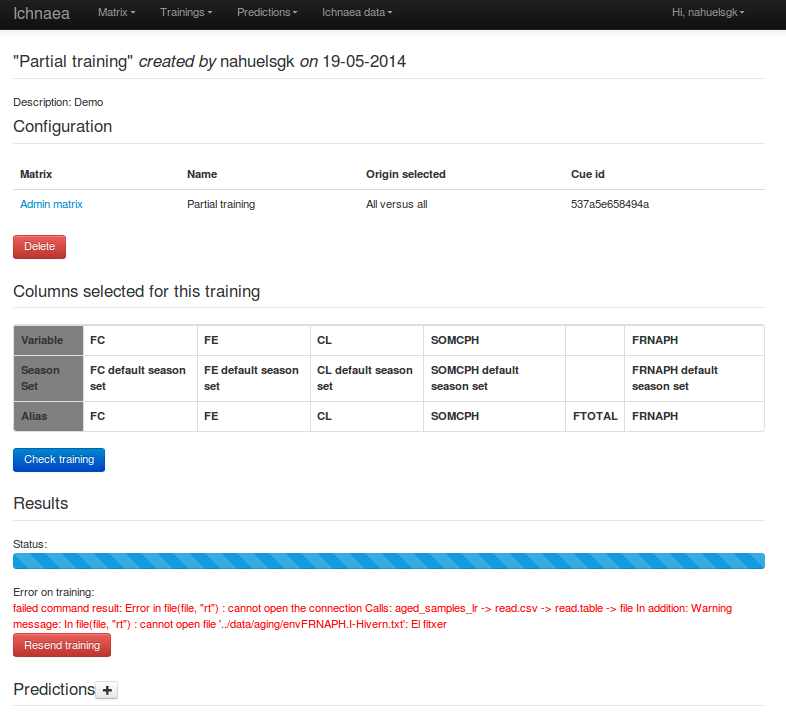
\includegraphics[scale=0.5]{img/userguide/view_training_pending.png}
  \caption{Interfície de visualització de entrenaments}
  \label{fig:viewTraining}
\end{figure}

\begin{itemize}
\item Títol: nom de l'entrenament, data de creació i propietari.
\item Configuracio: 
\begin{itemize}
\item Nom de la matriu com enllaç
\item Nom de l'entrenament
\item Origin-versus seleccionat(veure \ref{subsec:createtraining}).
\item \textbf{Cue id}: identificador del proces a la cua.
\end{itemize}
\item Columnes seleccionades per entrenar
\item Resultat: es una barra de progressió. Actualment Ichnaea no ens retorna estats parcial. Així que la barra estarà buida o plena.
\item Errors: errors capturats d'Ichnaea.
\item Prediccions: prediccions fetes amb aquest entrenament. Amb la icona \iconadd es pot crear una predicció usant aquest entrenament.
\end{itemize}

\section{Errors en els entrenaments}
Mirar la secció \ref{sec:ichnaeaErrors}.

\section{Prediccions}
\subsection{Crear una matriu de predicció a partir d'un entrenament desde un fitxer CSV o Excel}
Per crear una matriu de prediccions, primer s'ha de seleccionar un entrenament. Per seleccionar un entrenament i crear una predicció tenim 2 opcions:
\begin{itemize}
\item Opció a) Seguir el menú ''Trainings'' >> ''Create trainings'' >> Seleccionar un entrenament de la llista accedint amb l'icona \icontableninesquares.
\item Opcio b) Des de la interfície de visualitzacions d'entrenaments(mirar \ref{subsec:viewtraining}).
\end{itemize}
El format del fitxer es el mateix de que el que s'explica a l'apartat \ref{sec:create_matrix}. La principal diferencia es la resolució automàtica de configuracions de columnes: si el identificador de la columna es igual al identificador de la columna entrenada, automàticament s'assigna aquesta columna entrenada.

\subsection{Configuració d'una matriu de predicció}
A la figura \ref{fig:view_training_pending} es pot veure la interfície de configuració de les matrius.
\begin{figure}[h!]
  \centering
  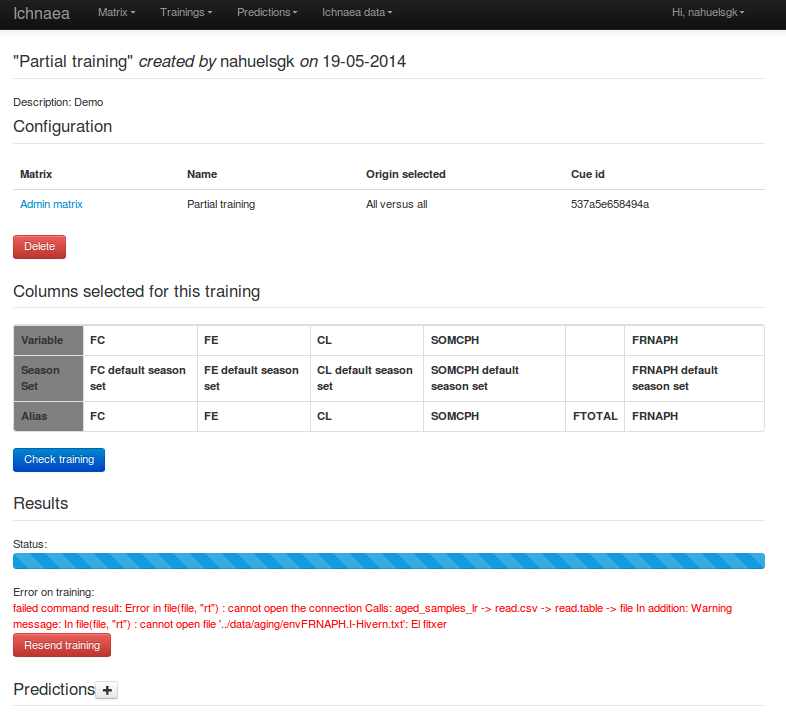
\includegraphics[scale=0.5]{img/userguide/view_training_pending.png}
  \caption{Interfície de visualització de entrenaments}
  \label{fig:view_training_pending}
\end{figure}
\textbf{Solament l'usuari propietari de la matriu la pot configurar}. A continuació descrivim les seccions de la interfície.

\subsubsection{Accions bàsiques}
Les accions bàsiques es troben a la part superior esquerre on:
\begin{itemize}
\item \iconremove esborra la matriu de predicció
\item \iconupdate per accedir a la interfície d'actualització de la matriu, on es pot actualitzar el nom i pujar tota nova matriu.
\item But\'{o} "Perform prediction" prepara les dades i les envia a la cua d'execucions de prediccions.
\end{itemize}

\subsubsection{Configuració de les dades de la matriu}
\paragraph{Columnes} Des de les columnes es configuren el mapejat amb les columnes entrenades on:
\begin{itemize}
\item \iconalias es per definir el alies de la columna
\item \iconvariable es per seleccionar la columna entrenada.
\end{itemize}

\paragraph*{Actualitzar una mostra} La actualització de mostres de prediccions es igual que la configuració de mostres de matrius, explicat a la pagina \pageref{matrixConfiguration}.

\paragraph*{Actualitzar una dada d'una fila i d'una columna} Es poden actualitzar les dades d'una mostra fent un doble ''click'' en una de les celles. Prement ''Enter'' es guarda el resultat.

\subsection{Executar una predicció}
Per executar una predicció mirar la secció anterior, a l'apartat ''Accions Basiques''. Una vegada enviat a execució es podra consultar a les prediccions de l'usuari(explicat a l'apartat \ref{subsec:myPrediccions}).

\subsection{Consultat resultats d'una prediccio}
Per consultar els resultats d'una predicció existeixen 2 formes:
\begin{itemize}
\item es pot accedir des de les prediccions de l'usuari(mirar l'apartat \ref{subsec:myPrediccions}) 
\item des de la interfície de configuració de la matriu de predicció mitjançant el but\'{o} ''View results'' en el cas que la la execució de la predicció hagi finalitzat.
\end{itemize}
La figura \ref{fig:viewresults} es la interfície de visualitzacions de resultats on:
\begin{itemize}
\item Informació bàsica: cont\'{e} enllaços a la matriu, l'entrenament, i la nova predicció.
\item Result: son cadascun dels resultats que retorna Ichnaea en una predicció. Actualment no s'interpreten aquests resultats. Simplement es recullen.
\end{itemize}
\begin{figure}[h!]
  \centering
  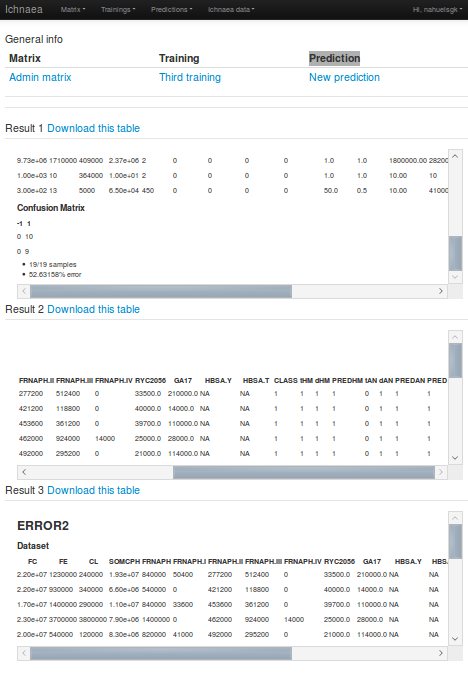
\includegraphics[scale=0.5]{img/userguide/result_prediction_gui.png}
  \caption{Interfície de visualització de resultats de prediccions}
  \label{fig:viewresults}
\end{figure}

\section{Problemes de Ichnaea}
\label{sec:ichnaeaErrors}
A traves de l'us de Ichnaea han sortit diversos errors a diferents nivells del software. Son externs a aquest projecte. Ichnaea encara esta evolucionant i l'aplicacio depen d'Ichnaea.

\subsection{Error en els entrenaments}
Si el proces d'entrenament llença un error, la aplicacio recull l'error i el mostra. Analitzen un exemple.\\

Actualment Ichnaea esta esperant trobar unes variables concretes. En el cas que no estiguin configurades en la matriu, Ichnaea donara un error del tipus que recull l'aplicació(figura \ref{fig:viewtrainingerror}).

\begin{center}
''failed command result: Error in file(file, "rt") : cannot open the connection Calls: aged\_samples\_lr - \> read.csv -> read.table -\> file In addition: Warning message: In file(file, "rt") : cannot open file '../data/aging/envFRNAPH.I-Hivern.txt': El fitxer ''
\end{center}

\begin{figure}[h!]
  \centering
  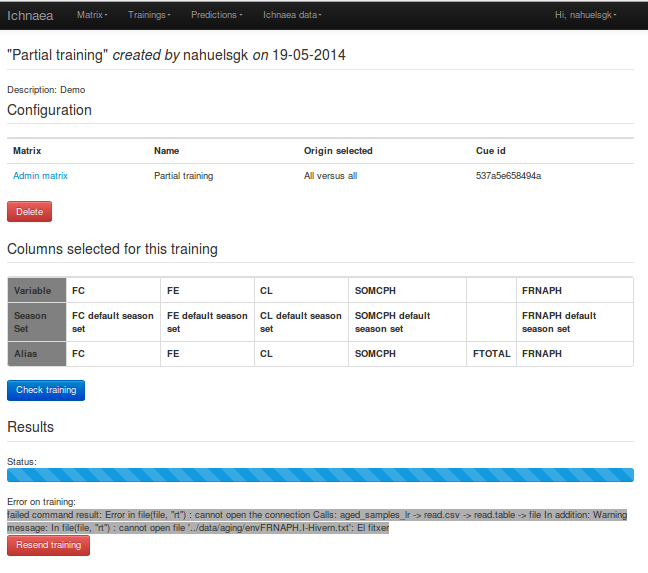
\includegraphics[scale=0.5]{img/userguide/error_training.png}
  \caption{Interfície de visualització d'entrenament amb error}
  \label{fig:viewtrainingerror}
\end{figure}
Una forma d'actuar envers a aquest error seria mirar la configuració de la matriu i mirar si existeix la columna FRNAPH.I.
